\textbf{TODO: find out laser parameters, LIA} 

\textbf{wie ausführlich allg.?}

\textbf{wie darauf eingehen, dass PCAs wahrscheinlich als emitter und detector eingesetzt werden??}

\textbf{variable gain, wie darauf eingehen?}

Generation and detection of THz radiation in a pulsed system were described in detail in Sections \ref{sec_gen_det}. Only a brief overview will be given here. The TSD setup (see Figure \ref{fig_TDS}) used for characterization of the fabricated H-Dipole antennas utilizes an ultrafast pulsed laser system with a pulse duration of \num{90} \si{\femto \s}, a repetition rate of \num{100} \si{\mega \hertz} and an optical wavelength of \num{1560} \si{\nano \meter}. The laser signal is coupled out using glass fibers. In order to achieve coherent signal detection, the THz-TDS setup utilizes a closed-loop system. Both the pump beam and the probe beam necessary for THz generation with PCAs are generated using the same laser beam. The THz signal is generated with the help of the pump beam and ultimately detected by sampling the temporal overlap of the probe beam and the THz field. This closed-loop approach ensures that the THz-TDS system provides high SNR and DNR. A beam splitter is utilized to split the initial laser pulse into the two needed signals. 

\textbf{TODO: Tx}

One of the pulses is directly coupled to the receiving port (Rx) of the setup. The receiver consists of an antenna that is being used to work as a recipient for THz radiation. For a PCA to work as a receiver, the device is illuminated by the femtosecond laser pulse, the probing pulse. By illuminating the device, free electron-hole pairs are generated. The incoming THz radiation which is to be measured biases the device. The illumination and biasing of the device results in a DC photocurrent. This current is proportional to the convolution of the incoming THz transient and the optical probing signal. The DC current can be read out by post detection electronics. 

\textbf{TODO: mehr zum receiver, evtl. noch auf Si-Linse eingehen}

As the measured photocurrent is generally very small (around $10^{-6} ... 10^{-9}$ \si{\ampere}), the signal is amplified by a trans-impedance amplifier (TIA).  With the TIA, gains of up to $\sim 10^7 $ \si{\volt}/\si{\ampere} can be achieved.

\begin{figure}[ht]
    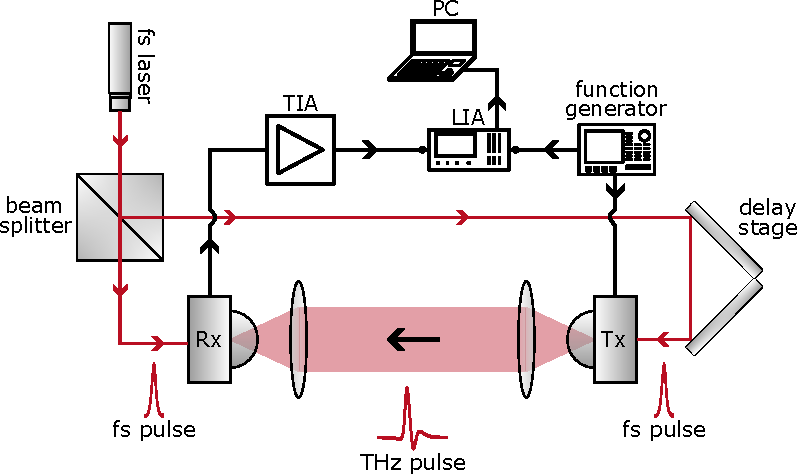
\includegraphics[width=0.9\linewidth]{figures/TDS_schematic.pdf}
    \centering
    \caption{Schematic diagram of the setup used for THz-TDS.}
    \label{fig_TDS}
\end{figure}

